

\section{Access token}
\label{win:access-token}
\index{Windows!Access Token}

Access token is a kernel data structure. What this means is only things in the kernel can touch this data. 
\begin{itemize}
    \item 
        \url{https://toxsec.com/windows-tokens/}
    \item
        \href{https://www.exploit-db.com/exploits/13054}{Security Implications of Windows Access Tokens - A Penetration Tester's Guide}
    \item 
        \href{https://www.elastic.co/blog/introduction-to-windows-tokens-for-security-practitioners}{Introduction to Windows tokens for security practitioners}
\end{itemize}


\subsection{Access token}

An Access token is an object that encapsulates the security identity of a process or thread. Windows uses access tokens when making security and access-related decisions. Access tokens store tamper-proof information about entities that can be put through access control lists. Further, these tokens are used during object access negotiation or when attempting privileged system tasks. Windows manages access tokens via the Local Security Authority Subsystem Service (LSASS)~\ref{windows:lsa}

Access tokens consist of:
\begin{itemize}
    \item The SID for the user’s account.
    \item A list of SIDs for security groups that include the user and the privileges held on the local computer by the user and the user’s security groups. This list includes SIDs both for domain-based security groups, if the user is a member of a domain, and for local security groups.
    \item The SID of the user or security group that becomes the default owner of any object that the user creates or takes ownership of.
    \item The SID for the user’s primary group.
    \item The default DACL that the operating system applies to objects created by the user if no other access control information is available.
    \item A list of privileges associated with the user’s account.
    \item The source, such as the Session Manager or LAN Manager, that caused the access token to be created.
    \item A value indicating whether the access token is a \emph{primary token}, which represents the security context of a process, or an \emph{impersonation token}, which is an access token that a thread within a service process can use to temporarily adopt a different security context, such as the security context for a client of the service.
    \item A value that indicates to what extent a service can adopt the security context of a client represented by this access token.
    \item Statistics about the access token that are used internally by the operating system.
    \item An optional list of SIDs added to an access token by a process to restrict use of the token.
    \item A logon session ID that indicates whether the token is associated with a Terminal Services client session. (The session ID also makes fast user switching possible because it contains a list of privileges.)
\end{itemize}


When a user authenticates to a Windows system, they are given an access token.  Any processes or threads initiated by the user will inherit a copy of the access token. Typically, this is known as the \emph{Primary Access Token}\label{win:primary-access-token}\index{win!Primary Access Token}. The system will use the primary access token of the thread requesting access to a resource unless the process is \emph{impersonating} another user. In that case, the system will use the process’s impersonation token.

{\bf Case of network authentication}:

The user’s logon session is unique to their workstation (as is their access token and privileges) and they cannot simply send their access token over the wire.

In this case, the user needs to {\bf re-authenticate} and establish a new logon session on the remote machine. For an interactive logon (and actually all other logon types like service, batch, etc., except network6) Windows will automatically cache the credentials as part of the Windows single sign-on (SSO) mechanism. This is the intended design of the Windows SSO mechanism and prevents the user from having to constantly re-enter their password when accessing network resources.

As a consequence, access tokens which link back to these types of logon sessions can authenticate to remote hosts and Windows will automatically authenticate on the users behalf whenever a network resource is accessed by a thread or process. Note that Windows will always use the credentials cached in the logon session that the access token is linked to when authenticating remotely.

Therefore, in order to establish a new logon session, the SMB server will need to authenticate the client over the network. In Windows domains, network authentication is typically performed via Kerberos or the legacy challenge-response protocol NTLM. Irrespective of the network authentication protocol used, on receiving an authentication request the target host will forward the credential information to the DC and, following successful authentication, establish a new network login session for the user (i.e., this login “represents a remote client”)

Network logins do not cache credentials and therefore you cannot use this token to authenticate to another remote host.

Most importantly from the server’s perspective, following the successful authentication of the remote user, it is presented with a newly minted access token which represents the network logon of the remote client. The diagram below illustrates this process:

\begin{figure}[!ht]
  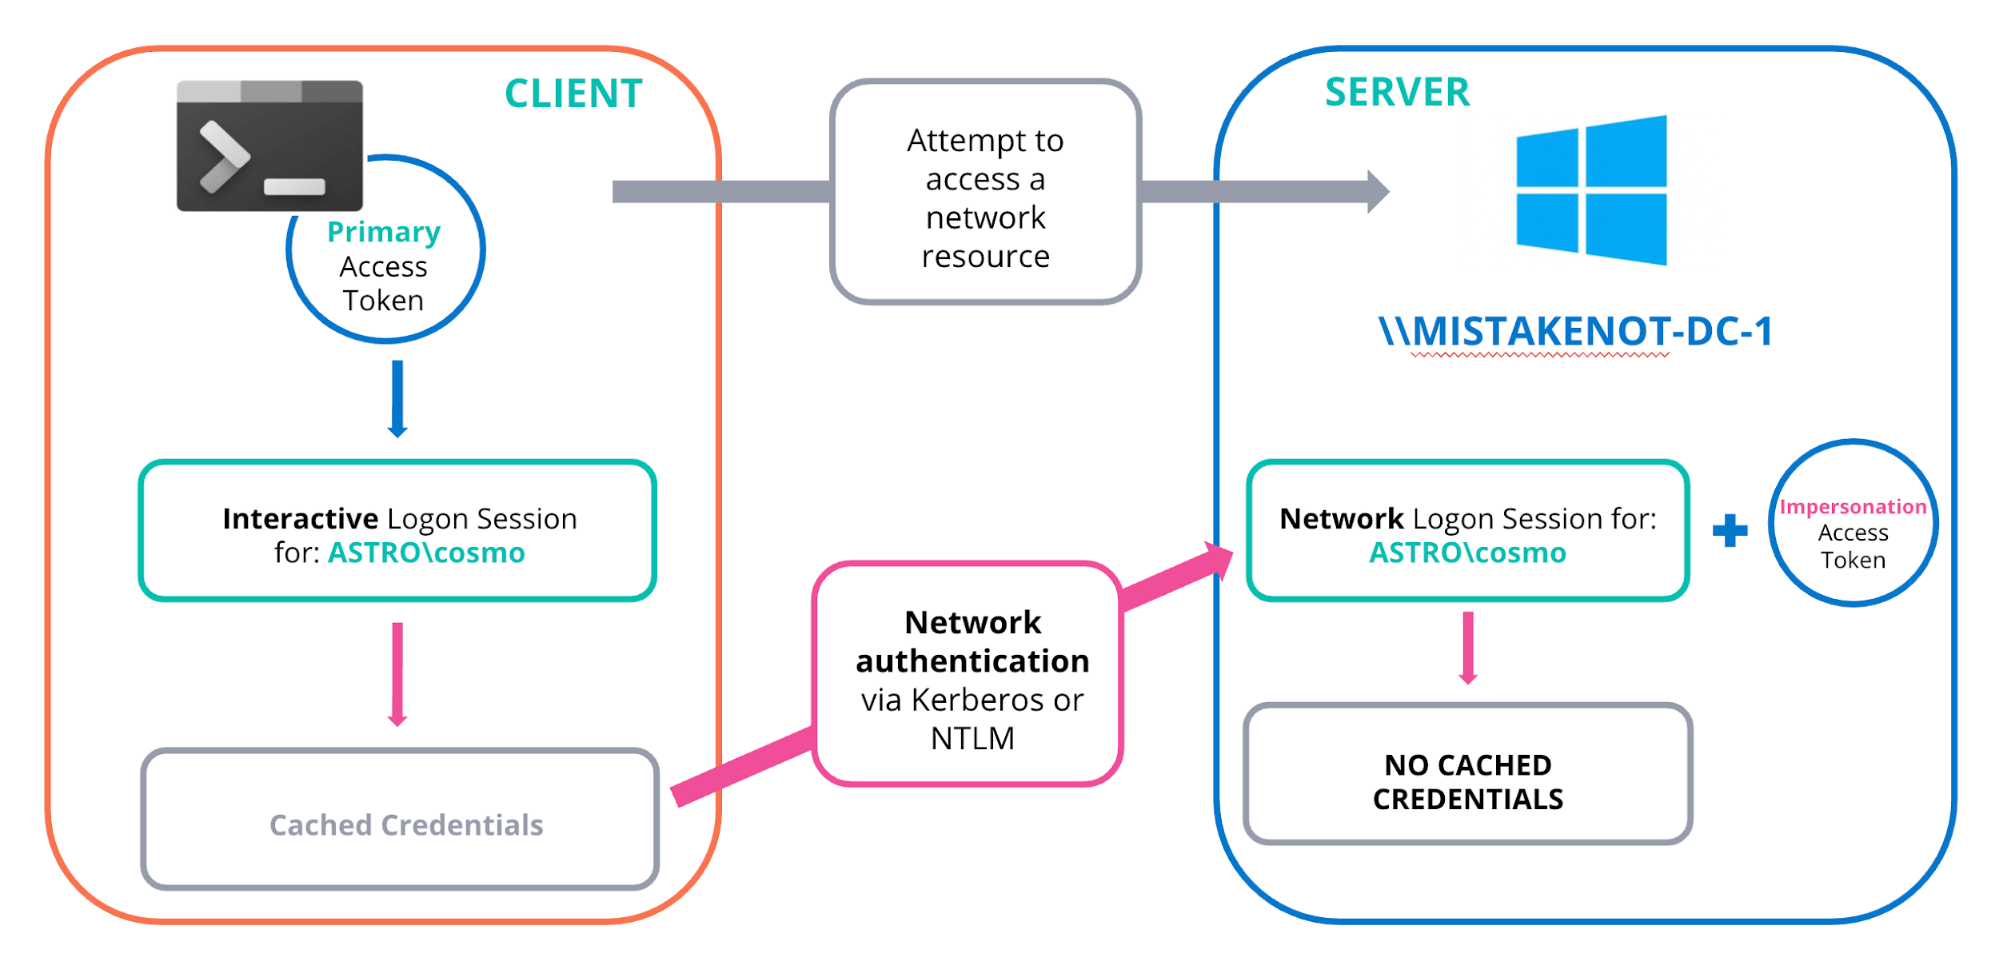
\includegraphics[width=\linewidth]{windows_knowledge/authorization/images/network-logon-tokens.png}
  \caption{Network Logon token}
    \label{fig:network-logon-token}
\end{figure}

In summary, from the perspective of a listening server process (say an SMB file server), the following steps must occur following a connection request from a remote client:
\begin{itemize}
    \item 
        The user is authenticated and a new logon session is created (\verb+NETWORK_ONLY+)
    \item 
        The server process is presented with a handle to an impersonation token which links back to the remote client’s new network logon session
    \item 
        The server can use this token to impersonate the client to perform work on their behalf
\end{itemize}

\subsection{Impresonation token}
An {\bf impersonation
token}\label{win:impresonation-token}\index{win!Impersonation Token} is an access token that is created to capture the security information of another agent. For example, if a server is doing a task on behalf of a client, the server is impersonating the client, and all operations will be performed under that client’s security context. Impersonation is simply the mechanism that allows a process to run by using the security credentials of another security object.

Keep in mind you may not add privileges to tokens after Windows generates them. Additionally, each sub-process generated by a thread inherited the parent process’s access token as-is. This is why there are times when a user may need to personate a token that belongs to them, but has a different set of privileges.

There are four impersonation levels:
\begin{itemize}
        \item \verb+SecurityAnonymous+ – The server cannot impersonate or identify the client.
        \item \verb+SecurityIdentification+ – With this, a server can get the identity and privileges of the client, but cannot impersonate the client.
        \item \verb+SecurityImpersonation+ – This impersonation level can impersonate the client’s security context on the local system.
        \item \verb+SecurityDelegation+ – The server can impersonate the client’s security context on remote systems.
\end{itemize}

Impersonation tokens can only be associated to threads, and they represent a client process's security subject. Impersonation tokens are usually created and associated to the current thread implicitly, by IPC mechanisms such as DCE RPC, DDE and named pipes.

\subsection{Restricted access token (filtered token)}
\label{win:filtered-token}

\href{https://docs.microsoft.com/en-us/windows/win32/secauthz/restricted-tokens}{Restricted
tokens} (also known as a filtered admin token) are a subset of primary or
impersonation tokens that have been modified to control privileges or
permissions. Restricted access tokens allow the system to remove privileges,
add deny-only access control entries, or perform other access rights changes.

Assuming User Account Control (UAC) is running during the initial token
creation process, LSA will attempt to identify if the user is a member of a
privileged group or has been granted a sensitive privilege using functionality
similar to the IsTokenRestricted function. Presence of a restricted SID will
result in a call to produce a new access token with reduced privileges.
